\documentclass[17pt]{beamer} %Makes presentation
%\documentclass[handout]{beamer} %Makes Handouts
\usetheme{Singapore} %Gray with fade at top
\useoutertheme[subsection=false]{miniframes} %Supppress subsection in header
\useinnertheme{rectangles} %Itemize/Enumerate boxes
\usecolortheme{seagull} %Color theme
\usecolortheme{rose} %Inner color theme

\definecolor{light-gray}{gray}{0.75}
\definecolor{dark-gray}{gray}{0.55}
\setbeamercolor{item}{fg=light-gray}
\setbeamercolor{enumerate item}{fg=dark-gray}

\setbeamertemplate{navigation symbols}{}
%\setbeamertemplate{mini frames}[default]
%\setbeamercovered{dynamics}
\setbeamerfont*{title}{size=\Large,series=\bfseries}
\setbeamerfont{footnote}{size=\tiny}

%\setbeameroption{notes on second screen} %Dual-Screen Notes
%\setbeameroption{show only notes} %Notes Output

\setbeamertemplate{frametitle}{\vspace{.5em}\bfseries\insertframetitle}
\newcommand{\heading}[1]{\noindent \textbf{#1}\\ \vspace{1em}}

\usepackage{bbding,color,multirow,times,ccaption,tabularx,graphicx,verbatim,booktabs}
\usepackage{colortbl} %Table overlays
\usepackage[english]{babel}
%\usepackage[latin1]{inputenc}
%\usepackage[T1]{fontenc}
\usepackage{lmodern}

%\author[]{Thomas J. Leeper}
\institute[]{
  \inst{}%
  Department of Government\\London School of Economics and Political Science
}

\usepackage{amsmath}
\usepackage{tikz}
\usetikzlibrary{shapes,arrows,decorations.pathreplacing,calc}

\title{Matching and Regression:\\Accounting for Rival Explanations}

\date[]{}

\begin{document}

\frame{\titlepage}

\frame{\tableofcontents}

\section[Exam]{Exam Preparation}
\frame{\tableofcontents[currentsection]}

\frame{
	
	\begin{center}
	\Large
	\textbf{What do you think will be on the exam?}
	\end{center}
	
}


\frame{
	\frametitle{Sample Paper}
	
	\url{https://moodle.lse.ac.uk/mod/resource/view.php?id=534210}
	
	\begin{itemize}
	\item ST Exam is 50\% of overall mark
		\begin{itemize}
		\item 25\%: 5 ``shorter answer'' questions (of 15); worth 5\% of total mark each
		\item 25\%: 1 essay (of 4)
		\end{itemize}
	\item Research Design Proposal is 50\% of overall mark
	\end{itemize}

}

\frame{}



\section[Regression]{Regression, Briefly}
\frame{\tableofcontents[currentsection]}


\frame{
	\frametitle{Uses of Regression}
	\begin{enumerate}\itemsep2em
	\item Description
	\item Prediction
	\item Causal Inference
	\end{enumerate}
}

\frame{
	\frametitle{Descriptive Inference}
	\begin{enumerate}\itemsep1em
	\item We want to understand a \textit{population} of cases
	\item We cannot observe them all, so:
		\begin{enumerate}
    		\item Draw a \textit{representative} sample
    		\item Perform mathematical procedures on sample data
    		\item Use assumptions to make inferences about population
    		\item Express uncertainty about those inferences based on assumptions
		\end{enumerate}
	\end{enumerate}
}

\frame{
	\frametitle{Parameter Estimation}
	\begin{itemize}\itemsep1em
    	\item We want to observe population \textit{parameter} $\theta$
    	\item If we obtain a representative sample of population units:\\
    		\begin{itemize}\itemsep1em
        		\item Our sample statistic $\hat{\theta}$ is an unbiased estimate of $\theta$
        		\item Our sampling procedure dictates how uncertain we are about the value of $\theta$
    		\end{itemize}
	\end{itemize}
}

\frame{

	\frametitle{Three Equations}
	\begin{enumerate}\itemsep1em
	\item Population:\\
		$Y = \beta_0 + \beta_1 X \hspace{0.5em} (+ \epsilon)$
	\item Sample estimate:\\
		$\hat{y} = \hat{\beta}_0 + \hat{\beta}_1 x$
	\item Unit:
		
		$y_i = \hat{\beta}_0 + \hat{\beta}_1 x_i + e_i$\\
		$y_i = \bar{y}_{0i} + (y_{1i} - y_{0i}) x_i + (y_{0i} - \bar{y}_{0i})$
	\end{enumerate}
}



\frame{

\frametitle{{\normalsize Mathematically, regression\dots}}

\small

\begin{itemize}\itemsep0.5em
\item<1-> \dots describes multivariate relationships in a sample of data points
\item<2-> \dots depending on sampling procedure, estimates those relationships in the population
\item<3-> \dots depending on model fit, provides a way to predict outcome values for new cases
\item<4-> \dots depending on model completeness, provides inferences about the effect of $X$ on $Y$
\end{itemize}

}


\section{Matching and Conditioning}
\frame{\tableofcontents[currentsection]}


\frame{
	Causal inference is about comparing an observed outcome to a counterfactual, ``potential outcome'' for the same cases

	Regression provides a ``statistical solution'' to the fundamental problem of causal inference (Holland)
}



\frame{

\frametitle{An Example}

\small

\begin{itemize}\itemsep0.5em
\item For example, if we think smoking might cause lung cancer, how would we know?
\vspace{0.5em}
\item How would we know if smoking caused lung cancer for an individual who smoked?
	\begin{itemize}
	\item What's the relevant counterfactual?
	\end{itemize}
\item How would we know if smoking causes lung cancer on average across many individuals?
	\begin{itemize}
	\item What's the relevant counterfactual?
	\end{itemize}
\end{itemize}

}


\frame{
\frametitle{Confounding}

\begin{itemize}
\item A source of ``endogeneity''
\item Synonyms: selection bias, omitted variable bias
\item In lay terms: the (non)correlation between $X$ and $Y$ does not reflect a causal relationship between $X$ and $Y$ are related for other reasons
	\begin{itemize}
	\item Most commonly: Some $Z$ causes both $X$ and $Y$
	\end{itemize}
\end{itemize}

}

\frame{

\frametitle{Addressing Confounding}

\begin{enumerate}\itemsep1em
\item<2-> Correlate a ``putative'' cause ($X$) and an outcome ($Y$)
\item<3-> Identify all possible confounds (\textbf{Z})
\item<4-> ``Condition'' on all confounds
	\begin{itemize}
	\item Calculate correlation between $X$ and $Y$ at each combination of levels of \textbf{Z}
	\end{itemize}
\end{enumerate}

}

% Mill's method of difference
\frame{
\frametitle{{\normalsize Mill's Method of Difference}}

\small

If an instance in which the phenomenon under investigation occurs, and an instance in which it does not occur, have every circumstance save one in common, that one occurring only in the former; the circumstance in which alone the two instances differ, is the effect, or cause, or an necessary part of the cause, of the phenomenon.
}



\frame<1-3>[label=smoking]{

\frametitle{Smoking Example}

\begin{enumerate}\itemsep0.5em
\item<2-> Partition sample into ``smokers'' ($X = 1$) and ``non-smokers'' ($X = 0$) 
\item<3-> Identify possible confounds
	\begin{itemize}
	\item Sex
	\item Parental smoking
	\item etc.
	\end{itemize}
\item<4-> Estimate difference in cancer rates between smokers and non-smokers within each group of \textit{covariates}
\end{enumerate}

}


\begin{frame}
\begin{center}
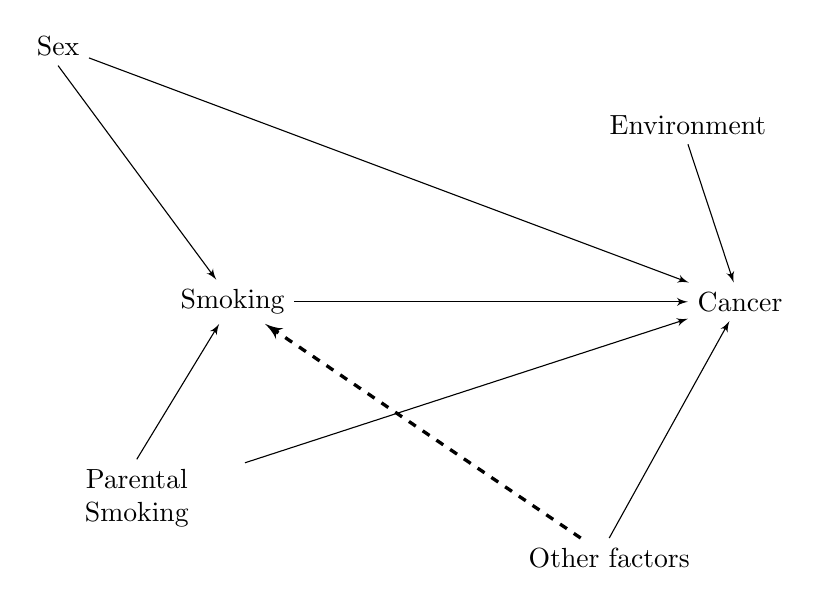
\begin{tikzpicture}[>=latex',circ/.style={draw, shape=circle, node distance=5cm, line width=1.5pt}]
    \draw[->] (0,0) node[left] (X) {Smoking} -- (5,0) node[right] (Y) {Cancer};
    \draw[->] (-3,3) node[above] (Z) {Sex} -- (X);
    \draw[->] (Z) -- (Y);
    \draw[->] (5,2) node[above] (A) {Environment} -- (Y);
    \draw[->] (4,-3) node[below] (E) {Other factors} -- (Y);
    \draw[->] (-2, -2) node[below, text width=2.5cm, align=center] (W) {Parental\\Smoking} -- (X);
    \draw[->] (W) -- (Y);
    \draw<2->[->, dashed, very thick] (E) -- (X);
\end{tikzpicture}
\end{center}
\end{frame}

\againframe<3->{smoking}

\frame{
\frametitle{Example I}
\begin{center}
\begin{tabular}{l r}
$X$ & $Y$ \textbf{(Cancer)} \\
Smokers & 0.15 \\
Non-smokers & 0.05 \\
\end{tabular}
\end{center}

\begin{align*}
ATE & = \bar{Y}_{X=1} - \bar{Y}_{X=0} \\
& = 0.15-0.05 \\
& = 0.10
\end{align*}

}

\frame{

\frametitle{Example II}
\begin{center}
\begin{tabular}{l l r}
$Z_1$ (Sex) & $X$ & $Y$ (Cancer) \\
0 & Smokers & \dots \\
0 & Non-smokers & \dots \\
1 & Smokers & \dots \\
1 & Non-smokers & \dots \\
\end{tabular}
\end{center}

\begin{align*}
ATE = & p_{\text{Male}} * (\bar{Y}_{X=1, Z_1 = 1} - \bar{Y}_{X=0, Z_1 = 1}) + \\
& p_{\text{Female}} * (\bar{Y}_{X=1, Z_1 = 0} - \bar{Y}_{X=0, Z_1 = 0})
\end{align*}

}


\frame{
\frametitle{Example III}

\footnotesize

\begin{center}
\begin{tabular}{l l l r}
$Z_2$ (Parent) & $Z_1$ (Sex) & $X$ & $Y$ (Cancer) \\
0 & 0 & Smokers & \dots \\
0 & 0 & Non-smokers & \dots \\
0 & 1 & Smokers & \dots \\
0 & 1 & Non-smokers & \dots \\
1 & 0 & Smokers & \dots \\
1 & 0 & Non-smokers & \dots \\
1 & 1 & Smokers & \dots \\
1 & 1 & Non-smokers & \dots \\
\end{tabular}
\end{center}

\tiny

\begin{align*}
ATE = & p_{\text{Male, Parent non-smoker}} * (\bar{Y}_{X=1, Z_1 = 1, Z_2=0} - \bar{Y}_{X=0, Z_1 = 1, Z_2=0}) + \\
& p_{\text{Female, Parent non-smoker}} * (\bar{Y}_{X=1, Z_1 = 0, Z_2=0} - \bar{Y}_{X=0, Z_1 = 0, Z_2=0}) + \\
& p_{\text{Male, Parent smoker}} * (\bar{Y}_{X=1, Z_1 = 1, Z_2=1} - \bar{Y}_{X=0, Z_1 = 1, Z_2=1}) + \\
& p_{\text{Female, Parent smoker}} * (\bar{Y}_{X=1, Z_1 = 0, Z_2=1} - \bar{Y}_{X=0, Z_1 = 0, Z_2=1}) + \\
\end{align*}

}

\frame{
\frametitle{Exact Matching}

\normalsize

\begin{itemize}\itemsep0em
\item Repeat this partitioning of the space into ``strata'' (or ``subclasses'')

\item Requires at least one ``treated'' and one ``untreated'' case at every combination of every covariate

\item More convenient notation:
	\vspace{-1em}

	\begin{align*}
	\text{Naive Effect} & = \bar{Y}_{X=1} - \bar{Y}_{X=0}\\
	\text{ATE} & = \bar{Y}_{X=1, \mathbf{Z}} - \bar{Y}_{X=0, \mathbf{Z}}
	\end{align*}

\end{itemize}

}


\frame{

\begin{center}
Note that matching is just a version of Mill's method of difference used for a large number of cases.
\end{center}


}


\frame{
	\frametitle{Omitted Variables}
	
	
	\footnotesize
	
	In the language of potential outcomes:\\
	
	{\footnotesize
	$\underbrace{E[Y_i| X_i = 1] - E[Y_i | X_i = 0] =}_{\text{Naive Effect}}$\\
	\vspace{1em}
	$\underbrace{E[Y_{1i}|X_i =1] - E[Y_{0i} | X_i = 1]}_{\text{Treatment Effect on Treated (ATT)}} + \underbrace{E[Y_{0i}|X_i = 1] - E[Y_{0i}|X_i=0]}_{\text{Selection Bias}}$
	}

	\vspace{1em}

	\footnotesize

	By conditioning, we assert that the potential (control) outcomes are equivalent between treated and non-treated cases, so the difference we observe between treatment and control outcomes is only the average causal effect of the ``treatment''.
}



\frame{

\frametitle{Caveat!}

\begin{itemize}\itemsep1em
\item We can only condition on \textit{observed} confounding variables
\item If we think other confounds might exist, but are unobservable, no form of conditioning can help us
	\begin{itemize}
	\item Example: Tobacco companies argued that an unknown genetic factor was a common cause of both smoking addiction and lung cancer
	\end{itemize}
\end{itemize}

}

\begin{frame}
\begin{center}
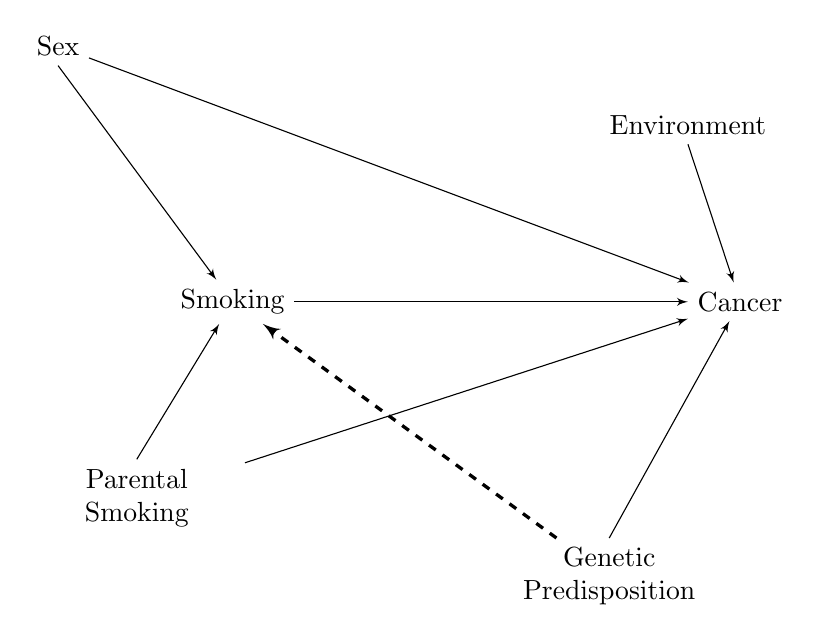
\begin{tikzpicture}[>=latex',circ/.style={draw, shape=circle, node distance=5cm, line width=1.5pt}]
    \draw[->] (0,0) node[left] (X) {Smoking} -- (5,0) node[right] (Y) {Cancer};
    \draw[->] (-3,3) node[above] (Z) {Sex} -- (X);
    \draw[->] (Z) -- (Y);
    \draw[->] (5,2) node[above] (A) {Environment} -- (Y);
    \draw[->] (4,-3) node[below, text width=3cm, align=center] (E) {Genetic\\Predisposition} -- (Y);
    \draw[->] (-2, -2) node[below, text width=2.5cm, align=center] (W) {Parental\\Smoking} -- (X);
    \draw[->] (W) -- (Y);
    \draw<2->[->, dashed, very thick] (E) -- (X);
\end{tikzpicture}
\end{center}
\end{frame}



\frame{

	\frametitle{Common Conditioning Strategies}
	\begin{enumerate}\itemsep1em
    	\item<2-> Condition on nothing (``naive effect'')
    	\item<3-> Condition on some variables
    	\item<4-> Condition on all observables
	\end{enumerate}
	\vspace{1em}
	\onslide<5->{Which of these are good strategies?}
}


\frame{
	\frametitle{Post-treatment Bias}
	\begin{itemize}\itemsep1em
	\item We usually want to know the \textbf{total effect} of a cause
	\item If we include a mediator, $D$, of the $X \rightarrow Y$ relationship, the coefficient on $X$:
		\begin{itemize}
    		\item Only reflects the \textbf{direct} effect
    		\item Excludes the \textbf{indirect} effect of $X$ through $D$
		\end{itemize}
	\item So don't control for mediators!
	\end{itemize}
}


% post-treatment example


\begin{frame}
\frametitle{Post-Treatment Bias}
\begin{center}
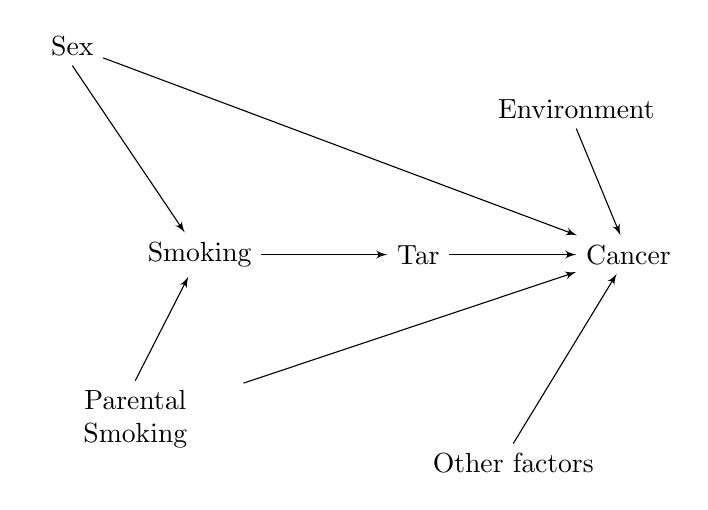
\begin{tikzpicture}[scale=0.8, >=latex',circ/.style={draw, shape=circle, node distance=5cm, line width=1.5pt}]
    \draw[->] (0,0) node[left] (X) {Smoking} -- (2,0) node[right] (D) {Tar};
    \draw[->] (D) -- (5,0) node[right] (Y) {Cancer};
    \draw[->] (-3,3) node[above] (Z) {Sex} -- (X);
    \draw[->] (Z) -- (Y);
    \draw[->] (5,2) node[above] (A) {Environment} -- (Y);
    \draw[->] (4,-3) node[below] (E) {Other factors} -- (Y);
    \draw[->] (-2, -2) node[below, text width=2.5cm, align=center] (W) {Parental\\Smoking} -- (X);
    \draw[->] (W) -- (Y);
    %\draw<2->[->, dashed, very thick] (E) -- (X);
\end{tikzpicture}
\end{center}
\end{frame}




\frame{
\frametitle{Post-Treatment Bias}

\small

\begin{center}
\begin{tabular}{l l r}
$D$ (Tar) & $X$ & $Y$ (Cancer) \\
0 & Smokers & \dots \\
0 & Non-smokers & \dots \\
1 & Smokers & \dots \\
1 & Non-smokers & \dots \\
\end{tabular}
\end{center}


\onslide<2->{Imagine:}

\vspace{-1em}

\footnotesize 
\begin{align*}
\onslide<2->{ATE_{\text{Tar}} = & (\bar{D}_{X=1} - \bar{D}_{X=0}) = 1}\\
\onslide<2->{ATE_{\text{Cancer} \text{ of Tar}} = & (\bar{Y}_{D=1} - \bar{Y}_{D=0}) = 1}\\
\onslide<4->{ATE_{\text{Cancer} \text{ of Smoking}} = & p_{D=1} (\bar{Y}_{X=1, D=1} - \bar{Y}_{X=0, D=1}) +\\
& p_{D=0} (\bar{Y}_{X=1, D=0} - \bar{Y}_{X=0, D=0})}\\
\end{align*}

}


\frame{}


\section{Multiple Regression}
\frame{\tableofcontents[currentsection]}


\frame{

\frametitle{Multiple Regression}

	\begin{itemize}\itemsep0.5em
	\item Regression achieves the same objectives as matching
		\begin{itemize}
		\item Estimate average causal of a variable conditional on other variables
		\end{itemize}
	\item Requires a \textit{linear} relationship between all RHS ($X$ variables) and $Y$
		\begin{itemize}
		\item Can be a set of binary indicator variables
		\end{itemize}
	\item We interpret coefficient estimates as \textit{marginal} average treatment effects
	\end{itemize}

}













\frame<1>[label=cis]{
\frametitle{{\normalsize Cusack, Iversen, and Soskice}}

\vspace{-1em}

\begin{center}
\small
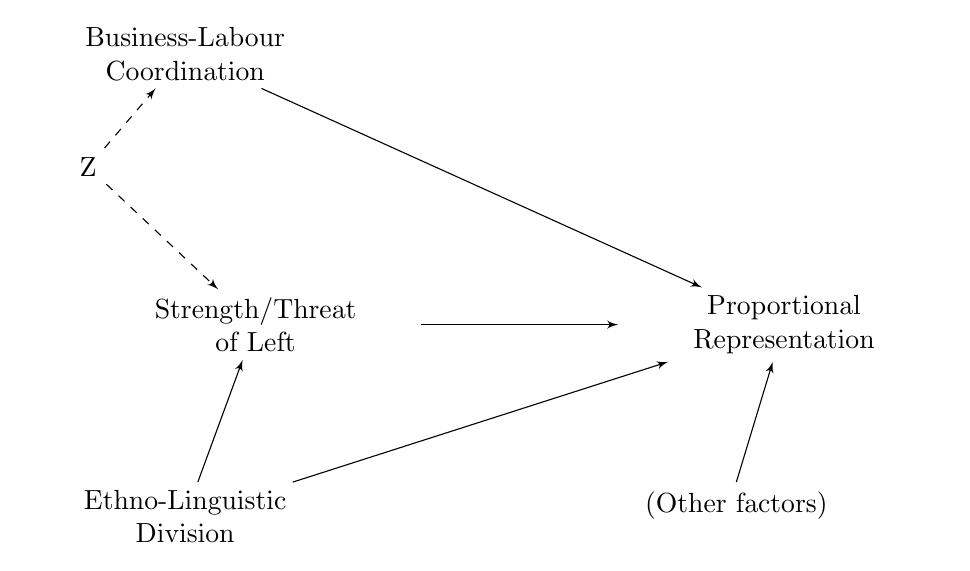
\begin{tikzpicture}[>=latex',n/.style={align=center, text width=4cm, inner sep=0, outer sep=3}]
    \draw<1-> (2.5,0) node[right,n] (Y) {Proportional\\Representation};
    \draw<1->[->] (4,-2) node[below] (E) {(Other factors)} -- (Y);
    \draw<1-> (-3, -2) node[below,n] (W) {Ethno-Linguistic\\Division};
    \draw<1->[->] (W) -- (Y);

    \draw<1,3->[->] (0,0) node[left,n] (X) {Strength/Threat\\of Left} -- (Y);
    \draw<1,3->[->] (W) -- (X);

    \draw<2-> (-3,3) node[above,n] (Z) {Business-Labour\\Coordination};
    \draw<2->[->] (Z) -- (Y);
        
    \draw<3-> (-4,2) node[left] (P) {Z};
    \draw<3->[->, dashed] (P) -- (X);
    \draw<3->[->, dashed] (P) -- (Z);
    
\end{tikzpicture}
\end{center}
}





% Rival hypotheses

\frame{
\frametitle{Testing Rival Hypotheses}

\small

\begin{itemize}\itemsep0.5em
\item Rival hypotheses can be derived from two (or more) different theories
\item We can conduct independent tests of each
	\begin{itemize}\footnotesize
	\item Is there evidence consistent with Hyp 1?
	\item Is there evidence consistent with Hyp 2?
	\end{itemize}
\item Regression allows us to test both simultaneously on the same data
	\begin{itemize}\footnotesize
	\item Is the data more consistent with Hyp 1 or Hyp 2?
	\end{itemize}
\item Draw inference about causality and about validity of theories based on data
\end{itemize}
}

\againframe<1->{cis}



\frame<1>[label=rival]{

\frametitle{Rival Theories}

\small

\begin{itemize}\itemsep0.5em
\item<1-> Rokkan--Boix:

\begin{equation}
PR = \beta_0 + \beta_1 Threat + \epsilon
\end{equation}

\item<2-> Cusack, Iversen, and Soskice:

\begin{equation}
PR = \beta_0 + \beta_2 Coordination + \epsilon
\end{equation}

\item<3-> Combined test:
\begin{equation}
PR = \beta_0 + \beta_1 Threat + \beta_2 Coordination + \epsilon
\end{equation}

\end{itemize}

}



\frame{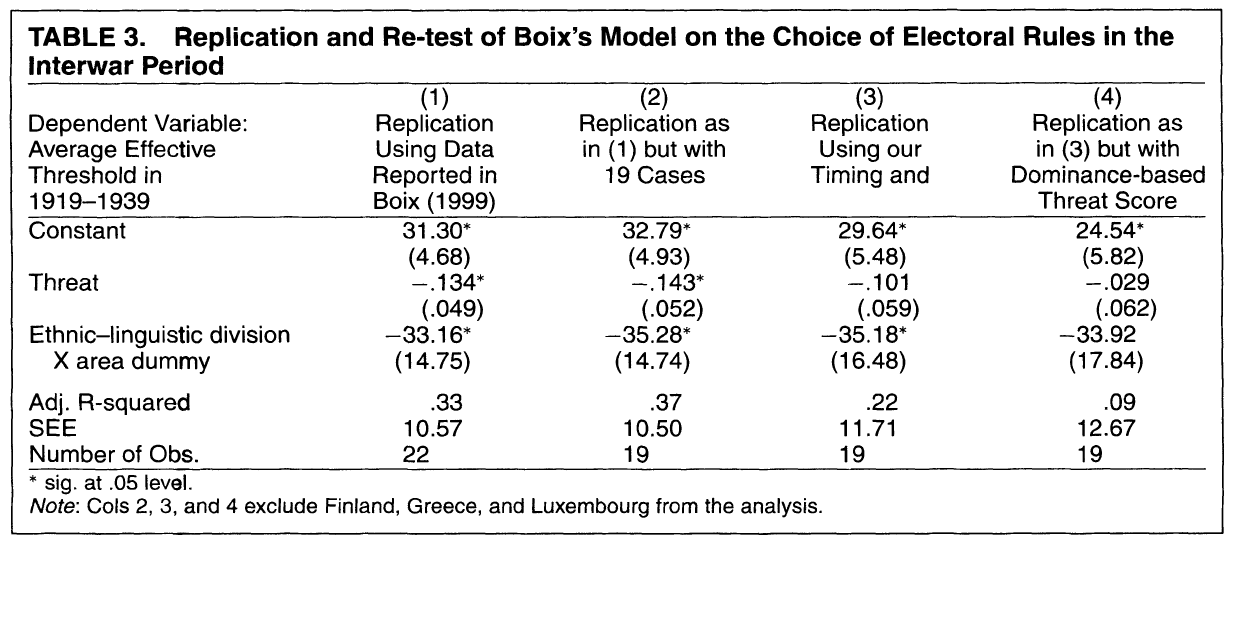
\includegraphics[width=\textwidth]{images/CusackIversenSoskiceTable3}}

\frame{
	\frametitle{Aside: Interpretation}
	\begin{itemize}\itemsep0.5em
	\item All our interpretation rules from earlier still apply in a multivariate regression
	\item Now we interpret a coefficient as an effect ``all else constant''
	\item Generally, not good to give all coefficients a causal interpretation
		\begin{itemize}
		\item Think ``forward causal inference''
		\item We're interested in the $X \rightarrow Y$ effect
		\item All other coefficients are there as ``controls''
		\end{itemize}
	\end{itemize}
}


\againframe<1-2>{rival}

\frame[label=table5]{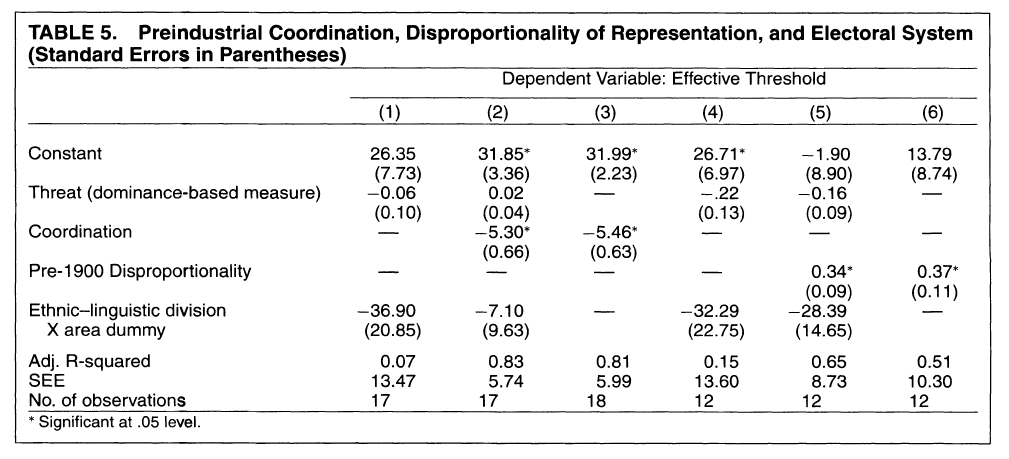
\includegraphics[width=\textwidth]{images/CusackIversenSoskiceTable5}}


\againframe<2-3>{rival}

\againframe{table5}


\frame{

\tiny
\begin{center}
\begin{tabular}{@{\extracolsep{5pt}}lcc} 
\\[-1.8ex]\hline 
%\hline \\[-1.8ex] 
% & \multicolumn{2}{c}{\textit{Dependent variable:}} \\ 
%\cline{2-3} 
%\\[-1.8ex] & \multicolumn{2}{c}{thresh} \\ 
\\[-1.8ex] & (1) & (2)\\ 
\hline \\[-1.8ex] 
 stthroct2 & 0.047 & 0.008 \\ 
  & (0.035) & (0.052) \\ 
  & & \\ 
 coordds & $-$6.019$^{***}$ & $-$5.284$^{***}$ \\ 
  & (0.706) & (1.008) \\ 
  & & \\ 
 dispro2 & 0.042 & 0.083 \\ 
  & (0.052) & (0.066) \\ 
  & & \\ 
 fragdum & 3.624 & 0.123 \\ 
  & (8.239) & (8.911) \\ 
  & & \\ 
 Constant & 28.239$^{***}$ & 25.211$^{***}$ \\ 
  & (5.866) & (6.565) \\ 
  & & \\ 
\hline \\[-1.8ex] 
Observations & 13 & 12 \\ 
R$^{2}$ & 0.947 & 0.948 \\ 
Adjusted R$^{2}$ & 0.920 & 0.919 \\ 
Residual Std. Error & 4.217 (df = 8) & 4.207 (df = 7) \\ 
F Statistic & 35.673$^{***}$ (df = 4; 8) & 32.084$^{***}$ (df = 4; 7) \\ 
\hline 
\hline \\[-1.8ex] 
\textit{Note:}  & \multicolumn{2}{r}{$^{*}$p$<$0.1; $^{**}$p$<$0.05; $^{***}$p$<$0.01} \\ 
\end{tabular}
\end{center}

}

\frame{

% ggplot(cis, aes(x = coordds, y = thresh))+ geom_jitter(width=0.3, height=1, size = 3, alpha = 0.5) + geom_smooth(method = "lm") + theme_bw()
\begin{center}
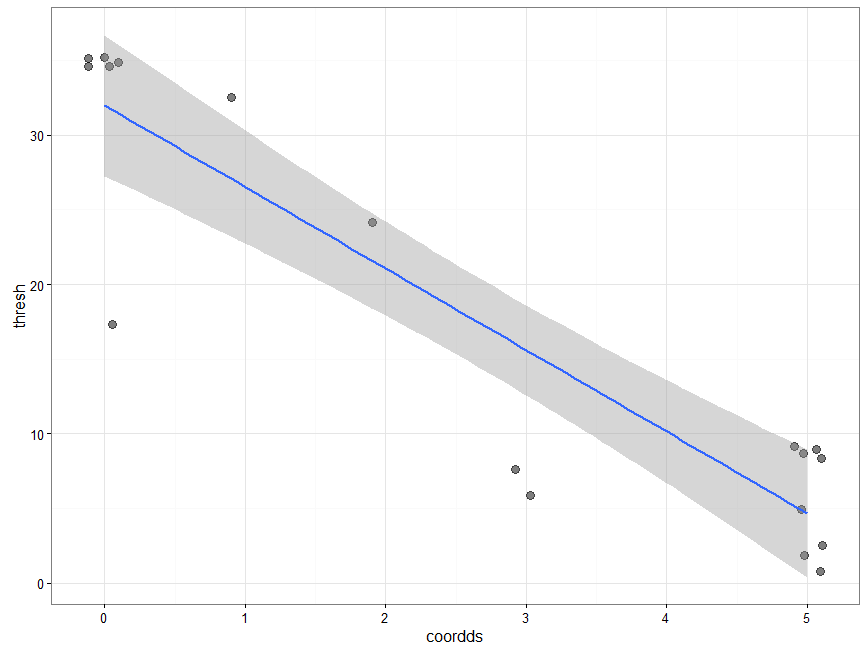
\includegraphics[width=\textwidth]{images/CISscatter}
\end{center}

}


\frame{

So the effect found by Rokkan and Boix was confounded by business--labour coordination. What was happening when they omitted the coordination variable?

}

\frame{
	\frametitle{Omitted Variable Bias}
	
	\small
	
	\begin{itemize}
	\item We want to estimate:
	\begin{align*}
	Y = \beta_0 + \beta_1 X + \beta_2 Z + \epsilon
	\end{align*}
	\item We actually estimate:
	\begin{align*}
	\tilde{y} & = \tilde{\beta_0} + \tilde{\beta_1} x + \epsilon\\
			  & = \tilde{\beta_0} + \tilde{\beta_1} x + (0 * z) + \epsilon\\
              & = \tilde{\beta_0} + \tilde{\beta_1} x + \nu
	\end{align*}
	\item Bias: $\tilde{\beta}_1 = \hat{\beta}_1 + \hat{\beta}_2 \tilde{\delta}_1$, where $\tilde{z} = \tilde{\delta}_0 + \tilde{\delta}_1 x$
	\end{itemize}
}



% further rival theories

\frame{

But have Cusack, Iversen, and Soskice considered all possible confounds?

}

\frame{

\begin{center}
\begin{tikzpicture}
\node[anchor=south west,inner sep=0] at (0,0) {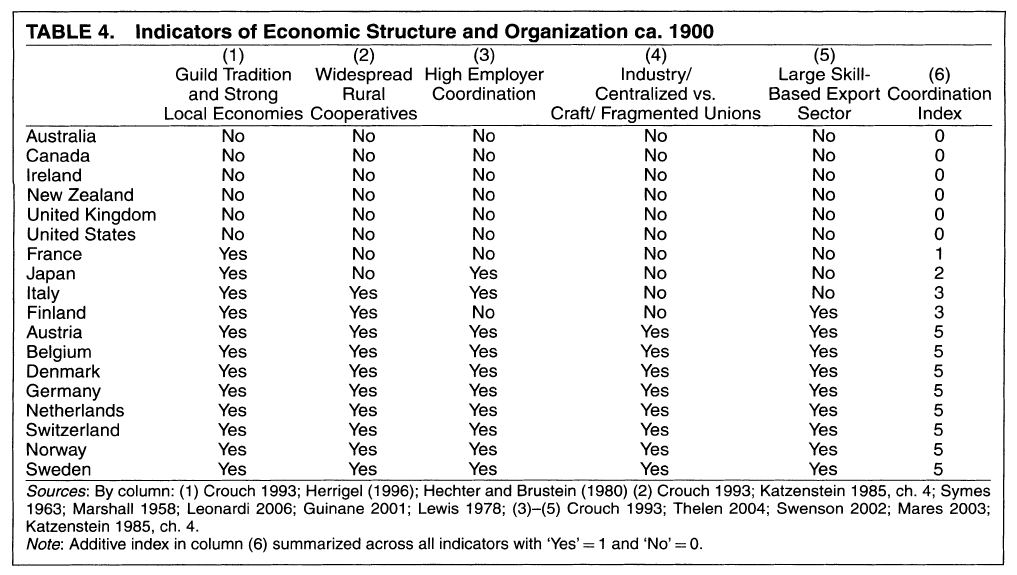
\includegraphics[width=\textwidth]{images/CusackIversenSoskiceTable4}};
\draw<2>[red,ultra thick,rounded corners] (0.15,3.5) rectangle (10.5,4.75);
\end{tikzpicture}
\end{center}

}


\frame{

\tiny

\begin{center}
\begin{tabular}{@{\extracolsep{5pt}}lcc} 
\\[-1.8ex]\hline 
%\hline \\[-1.8ex] 
% & \multicolumn{2}{c}{\textit{Dependent variable:}} \\ 
%\cline{2-3} 
%\\[-1.8ex] & \multicolumn{2}{c}{thresh} \\ 
\\[-1.8ex] & (1) & (2)\\ 
\hline \\[-1.8ex] 
 stthroct2 & 0.058 & 0.006 \\ 
  & (0.048) & (0.043) \\ 
  & & \\ 
 coordds & $-$5.556$^{***}$ & $-$0.398 \\ 
  & (1.578) & (2.467) \\ 
  & & \\ 
 dispro2 & 0.013 & $-$0.049 \\ 
  & (0.102) & (0.083) \\ 
  & & \\ 
 fragdum & 4.983 & 3.366 \\ 
  & (9.642) & (7.465) \\ 
  & & \\ 
 brit & 4.088 & 30.412$^{*}$ \\ 
  & (12.258) & (14.469) \\ 
  & & \\ 
 Constant & 26.911$^{***}$ & 9.390 \\ 
  & (7.388) & (9.253) \\ 
  & & \\ 
\hline \\[-1.8ex] 
Observations & 13 & 12 \\ 
R$^{2}$ & 0.948 & 0.970 \\ 
Adjusted R$^{2}$ & 0.910 & 0.945 \\ 
Residual Std. Error & 4.472 (df = 7) & 3.449 (df = 6) \\ 
F Statistic & 25.390$^{***}$ (df = 5; 7) & 39.083$^{***}$ (df = 5; 6) \\ 
\hline 
\hline \\[-1.8ex] 
\textit{Note:}  & \multicolumn{2}{r}{$^{*}$p$<$0.1; $^{**}$p$<$0.05; $^{***}$p$<$0.01} \\ 
\end{tabular}
\end{center}

}



\frame{}



\frame{
\frametitle{Two Lingering Issues}

\begin{enumerate}\itemsep1em

\item<2-> Inference to a population

	\begin{itemize}\itemsep0.5em
	\item Inferences from data to population depend on generalizability
	\item We may imagine that we are drawing from a ``superpopulation''
	\end{itemize}

\item<3-> Interactions, or effect \textit{heterogeneity}

	\begin{itemize}
	\item Interaction terms allow us to test whether than effect varies across values of a second variable
	
	\begin{align*}
	PR & = \beta_0 + \beta_1 Threat + \beta_2 Coordination + \epsilon \\
	   & = \beta_0 + \beta_1 Threat + \beta_2 Coordination + \beta_3 (Threat * Coordination) + \epsilon
	\end{align*}

	\item The interpretation of coefficient estimates changes!
	
	\end{itemize}

\end{enumerate}
}






\frame{}

\section*{Preview}

\frame{
\frametitle{Preview}

	\begin{itemize}\itemsep1em
	\item Next week: Experiments and Quasi-Experiments
	\item Following week: Research ethics
	\item Last week (Mar. 22):
		\begin{itemize}
		\item Research Design Proposal Due!
		\item Wrap-up course
		\end{itemize}
	\item I am on leave for 2 weeks from April 21
	\end{itemize}
}

\appendix
\frame{}


\end{document}
